\documentclass{article}
\usepackage{geometry}
\usepackage{amsmath}
\usepackage{graphicx}
\usepackage{enumitem}
\usepackage{bm}
\usepackage{float}
\usepackage{accents}
\usepackage{undertilde}

% added this to stop hbadness warning
\hbadness = 5000000

\geometry
{
	headheight = 4ex,
	includehead,
	includefoot,
	paper = a4paper,
	inner = 2.5cm,
	outer = 2.5cm,
	bindingoffset = 0.5cm,
	top = 2cm,
	bottom = 1.5cm
}


\title{\Huge Problem Set 3} 
\vspace{1cm}
\author {\Large Chara Tsirka 03315, Prodromos Avramidis 03291}

\begin{document}

\maketitle
\begin{center}
\vspace{1cm}

\includegraphics[width=0.3\textwidth]{uthlogo.png}
\vspace{2cm}
\end{center}
\begin{center}
  \Huge Neurofuzzy Computing \vspace{1cm}

  \Large Fall Semester 2023-2024 \vspace{1cm}

  \Large Professor: Dimitrios Katsaros
\end{center}


%Problem 1
\newpage
\noindent \textbf{Problem 1}

\noindent Design by hand (i.e., select manually the layers, the number of neurons per layer, the 
weights and biases per layers) an RBF network to perform the classification illustrated in 
the following figure. The network should produce a positive output whenever the input 
vector is in the shaded region and a negative output otherwise. Provide arguments for the 
selection of weights and biases
\begin{center}    
    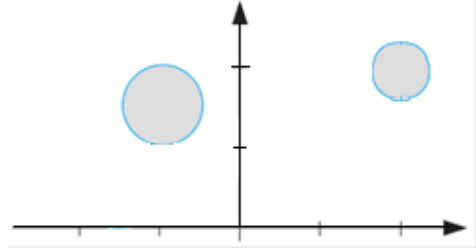
\includegraphics[width=0.4\textwidth]{pr1.png}
    \vspace{2cm}
\end{center}



\noindent \underline{\textbf{\textit{Solution:}}}


%Problem 2
\newpage
\noindent \textbf{Problem 2}

\noindent Write a MATLAB/python/… program to implement the steepest descent algorithm for the $ 1-S^1-1$ RBF network. 
Train the network to approximate the function:
\begin{center}
    $g(p) = 1 +sin(p*\pi/8) for -4 \leq p \leq 4$.    
\end{center}  

\begin{itemize}
    \item To train the network, select 30 data points at random from the interval $-4 \leq p \leq 4$.
    \item Initialize all parameters (weights and biases in both layers) as small random numbers, 
    and then train the network to convergence. (Experiment with the learning rate $\alpha$, to 
    determine a stable value.) Plot the network response for $-4 \leq p \leq 4$, and show the 
    training points on the same plot. Compute the sum squared error over the training 
    set. Use 4, 8, 12 and 20 centers. Try different sets of initial weights, different 
    sampling methods for selecting training pairs and record your observations. \\ \\
\end{itemize}

\noindent \underline{\textbf{\textit{Solution:}}}

\noindent random
Sum Squared Error with 4 centers: 1.617
Sum Squared Error with 8 centers: 0.22116
Sum Squared Error with 12 centers: 0.28262
Sum Squared Error with 20 centers: 0.29801

uniform
Sum Squared Error with 4 centers: 0.48242
Sum Squared Error with 8 centers: 0.048453
Sum Squared Error with 12 centers: 0.17237
Sum Squared Error with 20 centers: 0.044526

%Problem 3
\newpage
\noindent \textbf{Problem 3}

\noindent The net input expression for LVQ networks calculates the distance between the input 
and each weight vector directly, instead of using the inner product. The result is that the 
LVQ network does not require normalized input vectors. This technique can also be 
used to allow a competitive layer to classify non-normalized vectors. Such a network is 
shown in figure below.

\begin{center}
    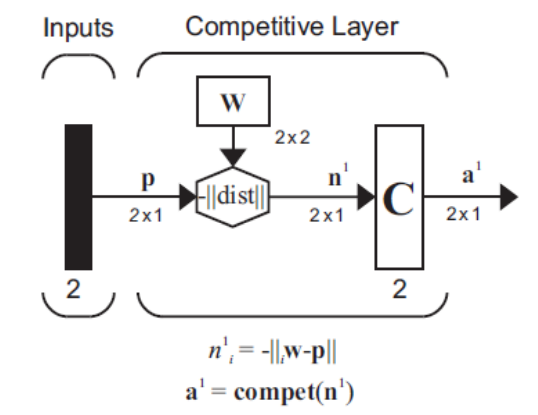
\includegraphics[width=0.4\textwidth]{pr3.png}
\end{center}

\noindent Use this technique to train a two-neuron competitive layer on the (non-normalized) 
vectors below, using a learning rate, $\alpha$, of 0.5 

\begin{center}
    $p_1 = \begin{bmatrix}
        1\\
        1
      \end{bmatrix}, p_2 = \begin{bmatrix}
        -1\\
        2
      \end{bmatrix}, p_3 = \begin{bmatrix}
        -2 \\
        2
      \end{bmatrix}$
\end{center}

\noindent Present the vectors in the following order: $p_1, p_2, p_3, p_2, p_3, p_1$. 
Here are the initial weights of the network: 

\begin{center}
    $w_1 = \begin{bmatrix}
        0\\
        1
      \end{bmatrix}, w_2 = \begin{bmatrix}
        1\\
        0
      \end{bmatrix}$
      \vspace{1cm}
\end{center}

\noindent \underline{\textbf{\textit{Solution:}}}

\noindent Presenting the vectors in the given order we get: \\\\ \underline{$p_1$:} \\\\$n_1^1 = -||w_1(0)-p_1|| = -1$ and $n_2^1 = -||w_2(0)-p_1|| = -1$ \\\\
$n_1^1 = n_2^1$, so $i^{*} = 1$ and $\alpha = \begin{bmatrix}
  1\\ 
  0
\end{bmatrix}$ \\\\ $w_1(1)=w_1(0) - \alpha(p_1-w_1(0)) = \begin{bmatrix}
  0 \\
  1
\end{bmatrix} + 0.5 (\begin{bmatrix}
  1\\
  1
\end{bmatrix} - \begin{bmatrix}
  0\\
  1
\end{bmatrix}) =  \begin{bmatrix}
  0.5\\
  1
\end{bmatrix}$
\\\\ \underline{$p_2$:} \\\\$n_1^2 = -||w_1(1)-p_2|| \approx -1.803$ and $n_2^2 = -||w_2(1)-p_2|| approx -2.829$ \\\\
$n_1^2 > n_2^2$, so $i^{*} = 1$ and $\alpha = \begin{bmatrix}
  0\\ 
  1
\end{bmatrix}$ \\\\ $w_2(1)=w_2(0) - \alpha(p_2-w_2(0)) = \begin{bmatrix}
  1 \\
  0
\end{bmatrix} - 0.5 (\begin{bmatrix}
  -1\\
  2
\end{bmatrix} - \begin{bmatrix}
  1\\
  0
\end{bmatrix}) =  \begin{bmatrix}
  2\\
  -1
\end{bmatrix}$
\newpage
\noindent\underline{$p_3$:} \\\\$n_1^3 = -||w_1(2)-p_3|| = -70$ and $n_2^3 = -||w_2(2)-p_3|| = -5$ \\\\
$n_1^3 > n_2^3$, so $i^{*} = 1$ and $\alpha = \begin{bmatrix}
  1\\ 
  0
\end{bmatrix}$ \\\\ $w_1(2)=w_1(1) - \alpha(p_3-w_1(1)) = \begin{bmatrix}
  0.5 \\
  1
\end{bmatrix} - 0.5 (\begin{bmatrix}
  -2\\
  2
\end{bmatrix} - \begin{bmatrix}
  0.5\\
  1
\end{bmatrix}) =  \begin{bmatrix}
  1.75\\
  0.5
\end{bmatrix}$
\\\\ \underline{$p_2$:} \\\\$n_1^4 = -||w_1(3)-p_2|| -3.13$ and $n_2^4 = -||w_2(3)-p_2|| \approx -4.24$ \\\\
$n_1^4 > n_2^4$, so $i^{*} = 1$ and $\alpha = \begin{bmatrix}
  1\\ 
  0
\end{bmatrix}$ \\\\ $w_1(3)=w_1(2) - \alpha(p_2-w_1(2)) = \begin{bmatrix}
  1.75 \\
  0.5
\end{bmatrix} - 0.5 (\begin{bmatrix}
  -1\\
  2
\end{bmatrix} - \begin{bmatrix}
  1.75\\
  0.5
\end{bmatrix}) =  \begin{bmatrix}
  0.375\\
  1.25
\end{bmatrix}$
\\\\\underline{$p_3$:} \\\\$n_1^5 = -||w_1(4)-p_3|| = -2.95$ and $n_2^5 = -||w_2(4)-p_3|| = -5$ \\\\
$n_2^5 > n_1^5$, so $i^{*} = 2$ and $\alpha = \begin{bmatrix}
  1\\ 
  0
\end{bmatrix}$ \\\\ $w_1(4)=w_1(3) - \alpha(p_3-w_1(3)) = \begin{bmatrix}
  0.375 \\
  1.25
\end{bmatrix} - 0.5 (\begin{bmatrix}
  -2\\
  2
\end{bmatrix} - \begin{bmatrix}
  0.375\\
  1.25
\end{bmatrix}) =  \begin{bmatrix}
  1.5625\\
  0.875
\end{bmatrix}$
\\\\ \underline{$p_1$:} \\\\$n_1^6 = -||w_1(5)-p_1|| = -0.57$ and $n_2^6 = -||w_2(5)-p_1|| = -2.23$ \\\\
$n_1^6 > n_2^6$, so $i^{*} = 1$ and $\alpha = \begin{bmatrix}
  1\\ 
  0
\end{bmatrix}$ \\\\ $w_1(5)=w_1(4) - \alpha(p_1-w_1(4)) = \begin{bmatrix}
  1.5625 \\
  0.875
\end{bmatrix} - 0.5 (\begin{bmatrix}
  1\\
  1
\end{bmatrix} - \begin{bmatrix}
  1.5625 \\
  0.875
\end{bmatrix}) \approx  \begin{bmatrix}
  1.28\\
  0.94
\end{bmatrix}$

%Problem 4
\newpage
\noindent \textbf{Problem 4}

\noindent Repeat Problem-03 for the following inputs and initial weights. Show the movements of 
the weights graphically for the first six each steps. If the network is trained for a large 
number of iterations, how will the three vectors be clustered in the final configuration?

\begin{center}
    $p_1 = \begin{bmatrix}
        2\\
        0
      \end{bmatrix}, p_2 = \begin{bmatrix}
        0\\
        1
      \end{bmatrix}, p_3 = \begin{bmatrix}
        2\\
        2
      \end{bmatrix}$\\
      \vspace{1cm}
      $w_1 = \begin{bmatrix}
        1\\
        0
      \end{bmatrix}, w_2 = \begin{bmatrix}
        -1\\
        0
      \end{bmatrix}$
      \vspace{1cm}

\end{center}

\noindent \underline{\textbf{\textit{Solution:}}}


%Problem 5
\newpage
\noindent \textbf{Problem 5}

\noindent You are asked to generate an Auto Regressive (AR) model and then create an RNN (such 
as LSTM, or GRU) that predicts it. Generate samples of an Auto Regressive model of 
the form: 
\begin{center}
    $X_t = a_1X_{t-1} + a_2X_{t-2} + a_3X_{t-3} + U_t$
    
\end{center}
where $a_1= 0.5, a_2= -0.1, a_3= 0.2$ and $U_t$ is independent-identically distributed Uniform in 
the interval (-0.25, 0.25). Now train an RNN of your choice that predicts the sequence. 

\begin{enumerate} [label=\Alph*]
    \item Apply the training algorithm on new samples and calculate the averaged cost square 
    error cost function. Investigate different number of training samples. (You are not 
    allowed to use your model knowledge when you design the RNN.)
    \item Optional part: You may use the Yule-Walker equations to compare your RNN 
    model. 
    
\end{enumerate}

\vspace{1cm}

\noindent \underline{\textbf{\textit{Solution:}}}


%Problem 6
\newpage
\noindent \textbf{Problem 6}

\noindent Consider the following Moving Average (MA) process:
\begin{center}
    $X_t = U_t + a_1U_{t-1} + a_2U_{t-2} + a_3U_{t-3} + a_4U_{t-4}+ a_5U_{t-5}+ a_6U_{t-6}$
\end{center}
\noindent where $a_1= a_2=5, a_3=a_4=a_5=a_6= -0.5$ and $U_t$ independent-identically distributed Uniform \\
(0, 0.5). 
Repeat the exercise above with a moving average model. \\ \\

\noindent \underline{\textbf{\textit{Solution:}}}



%Problem 7
\newpage
\noindent \textbf{Problem 7}

\noindent Model the following expressions as fuzzy subsets:
\begin{enumerate} [label = \Alph*]
    \item Large integers.
    \item Very small numbers.
    \item Medium-weight men.
    \item Numbers approximately between 10 and 20.
\end{enumerate}

\vspace{1cm}

\noindent \underline{\textbf{\textit{Solution:}}}\\
\begin{enumerate} [label = \Alph*]
  \item $\mu_{\utilde{A}}(x) = \begin{cases}
    0 &\text{for } x \leq 100 \\
    \frac{1}{1+\frac{1}{(x-100)^2}} &\text{for } x>100\\
    
  \end{cases}$, assuming that a large integer is an integer bigger than 100.\\\\
  \item $\mu_{\utilde{B}}(x) = \begin{cases}
    1 &\text{for } x \leq 0 \\
    \frac{1}{1+\frac{1}{(x-0.0001)^2}} &\text{for } x>100\\
  \end{cases}$ \\ \\
  \item $\mu_{\utilde{C}}(x) = 
    \frac{1}{1+\frac{1}{(x-75)^2}}$, assuming that a medium-weight man weights 75kg.\\\\
  \item $\mu_{\utilde{D}}(x) = \begin{cases}
    \frac{x^2}{100} & \text{for } x<10 \\
    1 &\text{for } 10 \leq x \leq 20 \\
    \frac{(x-30)^2}{100} &\text{for } x>20\\
    
  \end{cases}$,
\end{enumerate}


%Problem 8
\newpage
\noindent \textbf{Problem 8}

\noindent During the lectures, we have defined the concept of ordinary subset of level $\alpha$ of a fuzzy 
subset. The analogous definition, i.e., the ordinary relation of level $\alpha$ of a fuzzy relation, is 
straightforward. Determine analytically and show graphically the ordinary relation of level 
0.3 for the fuzzy relation with membership function: $\mu_{\utilde{R}}(x, y) = 1 - 1/(1+x^2+y^2)$.



%Problem 9
\newpage
\noindent \textbf{Problem 9}

\noindent Consider the reference set E= $[0, \alpha] \subset R$. If $\utilde{A}$ is the fuzzy subset defined by 
$\mu_{\utilde{A}}(x)$, give the index v of fuzziness of $\utilde{A}$ for:

\begin{enumerate} [label=\Alph*]
  \item $\mu_{\utilde{A}}(x)$ = $x^2/\alpha^2$, $x \in [0, \alpha].$
  \item $\mu_{\utilde{A}}(x) = 4x^2/\alpha^2$ if $0 \leq x\leq \alpha/2$ and $\mu_{\utilde{A}}(x) = 4(x-\alpha)^2/\alpha^2$ if $\alpha/2  <x \leq \alpha$
\end{enumerate}

\vspace{1cm}
\noindent \underline{\textbf{\textit{Solution:}}}


%Problem 10
\newpage
\noindent \textbf{Problem 10}

\noindent Determine analytically and show graphically the max-min composition of the two fuzzy 
relations $\utilde{R_1}$ and $\utilde{R_2}$ defined by the following membership functions:\\ \\ $\mu_{\utilde{R_1}} = e^{-k(x-y)^2}$, $k \geq 1$
\\ \\ $\mu_{\utilde{R_2}} = e^{-k(y-z)^2}$, $k \geq 1$

\vspace{1cm}
\noindent \underline{\textbf{\textit{Solution:}}}\\
\noindent The max-min composition of the two relations is: \\ \\
$\mu_{composition}(x,z) = max_y(min(e^{-k(x-y)^2}, e^{-k(y-z)^2}))$. \\ \\ \\Let's first analyze the inner part: $min(e^{-k(x-y)^2}, e^{-k(y-z)^2})$ \\ \\
In order to find the minimum we need to compare the two terms: \\ \\
$e^{-k(x-y)^2} = e^{-k(y-z)^2} \Rightarrow -k(x-y)^2 = -k(y-z)^2 \Rightarrow (x-y)^2 = (y-z)^2$, ($k \geq 1$) \\ \\
If both sides are if the same sign, then: \\ $x-y = y-z \Rightarrow y = \frac{x+z}{2}$.\\\\
If they are of different sign, then: \\ $x-y = z-y \Rightarrow x = z$.\\\\\\Now, we need to evaluate $min(e^{-k(x-y)^2}, e^{-k(y-z)^2})$ at these points: \\ \\
If $\bm{y = \frac{x+z}{2}}$, then $min(e^{-k(x-y)^2}, e^{-k(y-z)^2}) = e^{-k(x-\frac{x+z}{2})^2} = e^{-k\frac{(x-z)^2}{4}}$ \\ \\
If $\bm{x=z}$, then  $min(e^{-k(x-y)^2}, e^{-k(y-z)^2}) = e^{-k(z-y)^2}$. \\\\ So, $\mu_{composition}(x,z) = max(e^{-k\frac{(x-z)^2}{4}},  e^{-k(z-y)^2})$

\end{document}